\documentclass[10pt]{IEEEtran}
\usepackage[backend=biber,style=phys]{biblatex}
\usepackage{amsmath}
\usepackage{amsfonts}
\usepackage{amssymb}
\usepackage{caption}
\usepackage{graphicx}
\usepackage{hyperref}
\usepackage{hhline}
\usepackage{listings}
\usepackage{multirow}
\lstset{language=C++}
\usepackage{csquotes}
\usepackage{url} 
\graphicspath{{./images/}}
\addbibresource{betaspectroscopy.bib}

\begin{document}

% Define document title and author
    \title{$\beta$-Decay and $\gamma$-Ray Spectroscopy with NaI Detectors}
    \author{Jamison Lahman, Brandon Coleman, and Taylor Grueser
    \thanks{Instructor: Paul King}}
    \maketitle

% Write abstract here
\begin{abstract}
	Sodium-22 is an unstable isotope which decays through beta emission. In one instance, two 511 keV photons are emitted by positron annihilation in opposite directions to conserve momentum. In another instance, the an excited $^{22}$Ne atom emits a single, 1275 keV photon with no angular correlation. Using two or more particle detectors simultaneously, we were able to distinguish an angle dependency. We were able to confirm a sharp angle dependency for the 511 photon keV emission and the coincidence rate was random within error for the 1275-511 rate. Additionally, materials absorbed photon energy differently depending on the energy of the ray and the attenuation coefficients. Placing various materials between our sample and detector, we were able to experimentally measure the attenuation coefficients for energies of 511 keV and 1275 keV. For Copper, we found values of 0.7445$\pm$0.0083cm$^{-1}$ for a 551 keV photon and 0.4896$\pm$0.0077cm$^{-1}$ for a 1275 keV photon. Both of these are within one standard deviation of the literature values. For Aluminium, we found values of 0.4053$\pm$0.0024cm$^{-1}$ for a 551 keV photon and 0.1934$\pm$0.0055cm$^{-1}$ for a 1275 keV photon, neither of which are in agreement with literature values. 
\end{abstract}

\section{Introduction \& Theory}
Gamma rays are high energy photons which can be created during the decay process of radioactive elements such as $^{22}$Na. In the same way a single electron, which is held in orbit by electromagnetic forces, releases a photon as it falls to a lower energy orbit, the nucleus of an atom can release a photon as it falls to a lower energy state. Since the atom is held together by the strong-nuclear force, the energy is much greater than for changes in electronic states.

A common apparatus for measuring photons is called a scintillator. A scintillator works by converting the ionization energy of photons into visible light which can then easily be collected. Most scintillators are inorganic crystals doped with activating material, similar to doping in semiconductors. In this experiment, a NaI(Tl), sodium-iodide doped with thallium was employed. NaI detectors are commonly used because of their cheap cost to make\cite{nucleons}.

For $^{22}$Na, a positron is emitted from the atom. In its positron annihilation, two photons are emitted with nearly identical energies. In order to preserve Newton's laws of motion, the momentum of the two must be equal and opposite.
	\begin{equation}
		\frac{dp_1}{dt} = -\frac{dp_2}{dt}.	
	\end{equation}
Because of this conservation law, multiple detectors can be used to correlate a photon detection in one detector to an event in the other. The second photon emitted in the decay process in which the $^{22}$Na decays to the first excited state of $^{22}$Ne which produces one photon as it moves to the ground state and has no pair to conserve momentum and thus no angular correlation\cite{columbia}.

It is useful to know the mass attenuation coefficient, $\mu/\rho$, when calculating the energy deposition by photons in materials. Different materials absorb the energy of photons at various rates. The rate of absorption is also dependent on the energy of the photon. The mass attenuation coefficient determines how well the material absorbes the energy of an incoming photon. The densities of materials are well known\cite{density}, so multiplying by the density gets the attenuation coefficient (usually in units of cm$^{-1}$) which appears in the following exponential relation:
	\begin{equation}
		\frac{I}{I_0} = e^{-\mu x},
	\end{equation}
where $I$ is the intensity and $x$ is the length of the material traversed by the photon\cite{nucleons}.
\section{Experimental Details}
Our experimental setup followed Figure \ref{fig:setup}. We had our NaI detector connected to a photo-multiplier which was powered by an external voltage supply. From there, the signal was amplified again and then sent to the multichannel analyzer and processed on a computer. To ensure we were receiving a signal from our set-up, we plugged an oscilloscope into the output of the the multichannel analyzer.
    \begin{figure}[!hbt]
        \begin{center}
        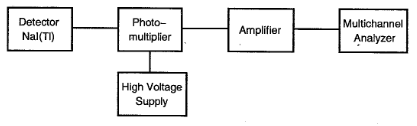
\includegraphics[width=\columnwidth]{setup}
        \caption{A simplified rendition of the experimental apparatus used\cite{nucleons}.}        
        \label{fig:setup}
        \end{center}
    \end{figure}

We had two detectors referred to as Gamma 1 and Gamma 2. Gamma 1 was a distance of 10.10$\pm$.05cm to the source while Gamma 2 was 10.30$\pm$.05cm. Gamma 1 is a type (7 D 4) detector while Gamma 2 is a type (6 D 4). Using the diagram in Figure \ref{fig:detector}, which describes the detectors used in the experiment, these correspond to diameters of 2.00 and 1.75 inches respectively. The diameter and the distance of the detector from the source both contribute to the solid angle, $\Omega$. $N_0$ is simply the rate of emission from the sample.
The detection rate of the detector, R, is given by the relation\cite{columbia},
	\begin{equation}
		R = N_0 \frac{\Omega}{4\pi}.
	\end{equation}
    \begin{figure}[!hbt]
        \begin{center}
        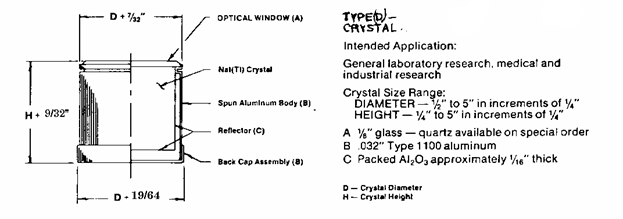
\includegraphics[width=\columnwidth]{GMAimage012}
        \caption{Detector schematic for the NaI detectors\cite{harshaw}.}        
        \label{fig:detector}
        \end{center}
    \end{figure}   

Since $\Omega$ has an angle and radial dependency, the angle correlation will vary slightly with different radial components though this is will not be examined in this study. For example, a detector extremely close to a sample might not see any change with respect to a change in angle as the the radial component dominates in the solid angle calculation. The detectors are considered far enough from the sample to have adequate angle resolution while maintaining an adequate signal.

The gain of Gamma 1 was set to 450 while Gamma 2 was set to 266. For our gates, we set $g_0$ on the interval [160,290], $g_1$ on the interval [190,350], and $g_2$ on the interval [530,715].

For the attenuation coefficient calculations, aluminium and copper sheets were used. Each sheet had a thickness of 1.270$\pm$0.079cm

\section{Data}

To perform a rough energy calibration, we took data at 180$^\circ$ with no material obstructing the photon's paths at the beginning of each day for a total of six samples over three days. The peaks are roughly Poisson distributions so the error on of the mean is only dependent on the RMS of the peak and the number of counts, N\cite{bevington}:

	\begin{equation}
		\sigma_{\bar{x}} = \frac{\sigma_x}{\sqrt{N}}.
	\end{equation}
	
The detectors are going to have energy calibrations which are independent of each other, so each must be calibrated separately. In all cases, the background was subtracted automatically using the program ROOT.
    \begin{table}[!hbt]
        \begin{center}
        \begin{normalsize}Data for Gamma 1 Energy Calibration\end{normalsize}
        \begin{tabular}{|c|c|c|c|c|}
			\hline        	
        	Bin Peak & Time (s) & Total Counts & RMS & $\sigma_{\bar{x}}$ \\    
            \hline
            285.1 & 600 & 34187 & 18.08 & 0.098 \\
            \hline
            284.8 & 300 & 23817 & 17.75 & 0.12 \\
            \hline
            284.7 & 600 & 49067 & 18.04 & 0.081 \\
            \hline
            284.3 & 600 & 49095 & 18.06 & 0.082 \\
            \hline
            359.8 & 450 & 1030 & 27.98 & 0.87 \\
            \hline
            667.4 & 600 & 4586 & 26.95 & 0.098 \\
            \hline
            666.5 & 300 & 3208 & 29.1 & 0.51 \\
            \hline
            666.5 & 600 & 6605 & 28.32 & 0.35 \\
            \hline
            666.0 & 600 & 6507 & 26.03 & 0.32 \\
            \hline
       \end{tabular}
       \caption{The 285 bin peak corresponds to the 511 keV photons from $^{22}$Na while the 666 peak corresponds to the 1275 keV photons. The 360 peak is the 662 keV photon of decaying $^{137}$Cs\cite{sonzogni}.}
       \label{tab:gam1}
       \end{center}
    \end{table}
    
    \begin{table}[!hbpt]
        \begin{center}
          \begin{normalsize}Data for Gamma 2 Energy Calibration\end{normalsize}
          \begin{tabular}{|c|c|c|c|c|}
			\hline        	
        	Bin Peak & Time (s) & Total Counts & RMS & $\sigma_{\bar{x}}$ \\    
            \hline
            259.5 & 600 & 19129 & 13.89 & 0.10 \\
            \hline
            259.1 & 300 & 13174 & 14.30 & 0.12 \\
            \hline
            254.9 & 600 & 24614 & 13.69 & 0.087 \\
            \hline
            258.4 & 600 & 24864 & 13.80 & 0.088 \\
            \hline
            328.1 & 450 & 604 & 16.33 & 0.66 \\
            \hline
            612.9 & 600 & 2601 & 21.99 & 0.43 \\
            \hline
            614.9 & 300 & 1767 & 21.00 & 0.50 \\
            \hline
            609.2 & 600 & 3293 & 20.68 & 0.36 \\
            \hline
            612.8 & 600 & 3300 & 21.36 & 0.37 \\
            \hline
          \end{tabular}
          \caption{The peak bin numbers corresponds to similar photon energies as Table \ref{tab:gam1}.}
          \label{tab:gam2}
       \end{center}
    \end{table}    

    Plotting the literature energy\cite{sonzogni} as a function of the peak bin number yields Figure \ref{fig:cal},
   
    \begin{figure}[!hbpt]
        \begin{center}
        \normalsize{Energy Calibration of NaI Detectors}
        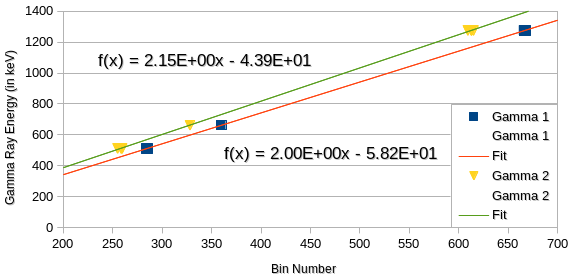
\includegraphics[width=\columnwidth]{Cal}
        \caption{A rough energy calibration the NaI detectors using decay peaks from $^{22}$Na and $^{137}$Cs. Data is taken from Tables \ref{tab:gam1} and \ref{tab:gam2}. The residuals are plotted in Figures \ref{fig:calres1} and \ref{fig:calres2}.}    
        \label{fig:cal}
        \end{center}
    \end{figure}
Performing a least-squares linear regression on the data in Figure \ref{fig:cal} yields the following energy calibrations for Gamma 1 and Gamma 2 respectively:

\begin{eqnarray*}
y = (1.9995\pm 0.0010)x-(58.22\pm 0.32), \text{cov}=-3.1648\text{E-4} \\
y = (2.1535\pm 0.0013)x-(43.90\pm 0.36), \text{cov}=-4.3965\text{E-4} \\
\end{eqnarray*}

    To find the angle correlations, we simply integrate the number of similar incidences which occur simultaneously in both detectors while varying the angle between the detectors as seen in Figures \ref{fig:511-511}, \ref{fig:511-1275}, and \ref{fig:1275-511}. Since the peaks are Poisson distributions, the error is simply\cite{bevington}  
    \begin{equation}
  		\sigma_N = \sqrt{N}.
    \end{equation}
\begin{center}
    \begin{table}[!hbpt]
        \begin{center}
        \normalsize{Angle Correlation for Each Photon}
        \begin{tabular}{|c|c|c|c|c|}
			\hline        	
        	Angle ($^\circ$) & 511-511 & 511-1275 & 1275-511 & 1275-1275 \\    
            \hline
            180.0 & 11145 & 42 & 34 & 0 \\
            \hline
            175.0 & 8272 & 27 & 41 & 0 \\
            \hline
            165.0 & 775 & 28 & 29 & 0 \\
            \hline
            150.0 & 108 & 18 & 29 & 0 \\
            \hline
            130.0 & 67 & 37 & 31 & 0 \\
            \hline
            110.0 & 81 & 34 & 35 & 0 \\
            \hline
            90.0 & 58 & 24 & 31 & 0 \\
            \hline
       \end{tabular}
       \caption{The angle measurements were taken in the anti-clockwise direction of Gamma 1 to Gamma 2. The first number represents which portion of the energy spectrum being recorded by Gamma 1 while the second number is similar for Gamma 2. The values indicate the number of coincidences detected in both detectors simulations.}
       \label{tab:angle}
    \end{center}
\end{table}        
	
    \begin{figure}[!hbtp]
    			\center{\normalsize{Number of 511-511 Coincidences}}
		   	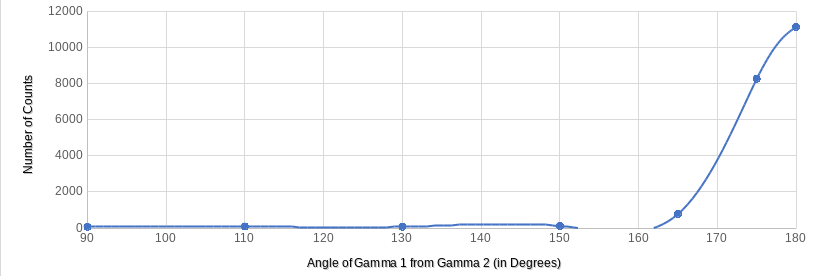
\includegraphics[width=\linewidth]{511-511}
			\caption{The number of incidences in Gamma 1 which correspond to an event in Gamma 2 for the 511 keV photon regime as a function of angle between the detectors. The number of coincidences at each angle can help us determine whether or not the photons have an angle dependence between them.}
			\label{fig:511-511}
    \end{figure}
\end{center}
    \begin{figure}[!hbtp]
    			\center{\normalsize{Number of 511-1275 Coincidences}}
			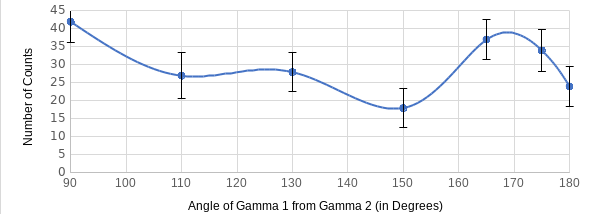
\includegraphics[width=\linewidth]{511-1275}
			\caption{The number of photons around the 511 keV photon incident in Gamma 1 which correspond to 1275 photon event in Gamma 2.  The number of coincidences at each angle can help us determine whether or not the photons have an angle dependence between them.}
			\label{fig:511-1275}
    \end{figure}     
    \begin{figure}[!hbtp]
    			\center{\normalsize{Number of 1275-511 Coincidences}}
			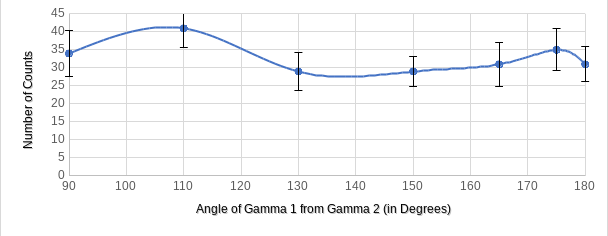
\includegraphics[width=\linewidth]{1275-511}
			\caption{The number of photons around the 1275 keV peak incident in Gamma 1 which correspond to 511 photon event in Gamma 2. The number of coincidences at each angle can help us determine whether or not the photons have an angle dependence between them.}
			\label{fig:1275-511}    
    \end{figure} 

To find the attenuation coefficients for given materials, we measured the intensity of the peaks, i.e. the total number of counts after background subtraction, with various amount of thickness of material in between the source and the detectors.       

Again the peaks are Poisson distributions so Eqn. (5) applies. Converting the errors to log-space, we find
    \begin{equation}
    	\epsilon = \frac{\sigma_N}{I}.
    \end{equation}
    \begin{center}
    \begin{table}[!hpbt]
      \begin{center}
        \normalsize{Attenuation Through Copper for 511 keV Photon}
        \begin{tabular}{|c|c|c|c|c|}	
		   \hline        	
		   Detector & Thickness (cm) & Intensity & $ln(I/I_0$) & $\epsilon$ \\
            \hline
            \multirow{4}{*}{Gamma 1} & 0 & 47634 & 0 & 0.0032 \\
            \hhline{~----}
	        & 1.270 & 18336 & -0.9547 & 0.0074 \\
	        \hhline{~----}
            & 2.540 & 6699 & -1.962 & 0.012 \\
            \hhline{~----}
            & 3.810 & 2742 & -2.855 & 0.019 \\
            \hline
            \multirow{3}{*}{Gamma 2} & 0 & 26348 & 0 & 0.0043 \\
            \hhline{~----}
            & 1.270 & 10587 & -0.912 & 0.010 \\
            \hhline{~----}
            & 2.540 & 4268 & -1.820 & 0.018 \\
            \hline
       \end{tabular}
       \caption{The intensity is simply the number of incidences detected by our detector. $I_0$ is the intensity with no material in between the source and detector. $\epsilon$ is the error in log-space as defined by Eqn. (6).}
       \label{tab:copper511}
      \end{center}
    \end{table}  
    \begin{figure}[!hbpt]
			\center{\normalsize{Attenuation Through Copper for 511 keV Photon}}
			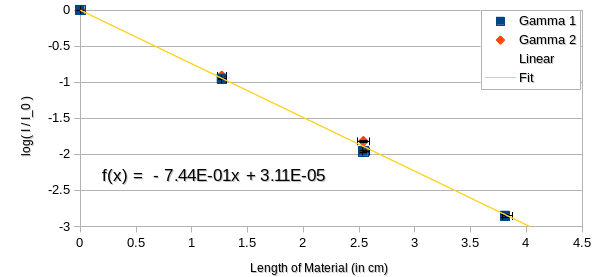
\includegraphics[width=\linewidth]{Attenuation511Cu}
			\caption{The following graph shows the number of counts in their respective detector as a function of the thickness of the material in between the source and the detector. The slope tells us the attenuation coefficient of the material.}
			\label{fig:511Cu}
    \end{figure}  
\end{center}
 
    \begin{table}[!hbtp]
      \begin{center}
        \normalsize{Attenuation Through Copper for 1275 keV Photon}
        \begin{tabular}{|c|c|c|c|c|}	
		   \hline        	
		   Detector & Thickness (cm) & Intensity & $ln(I/I_0$) & $\epsilon$ \\
            \hline
            \multirow{4}{*}{Gamma 1} & 0 & 64616 & 0 & 0.0088 \\
            \hhline{~----}
	        & 1.270 & 2814 & -0.824 & 0.019 \\
	        \hhline{~----}
            & 2.540 & 1858 & -1.239 & 0.023 \\
            \hhline{~----}
            & 3.810 & 1046 & -1.814 & 0.031 \\
            \hline
            \multirow{3}{*}{Gamma 2} & 0 & 3534 & 0 & 0.012 \\
            \hhline{~----}
            & 1.270 & 1947 & -0.596 & 0.023 \\
            \hhline{~----}
            & 2.540 & 1127 & -1.143 & 0.030 \\
            \hline
       \end{tabular}
       \caption{The intensity is simply the number of incidences detected by our detector. $I_0$ is the intensity with no material in between the source and detector. $\epsilon$ is the error in log-space as defined by Eqn. (6).}
       \label{tab:copper1275}
      \end{center}
    \end{table}  
    \begin{figure}[!hpbt]
        \begin{center}
			\normalsize{Attenuation Through Copper for 1275 keV Photon}
			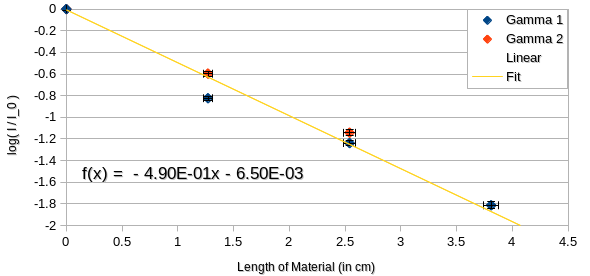
\includegraphics[width=\linewidth]{Attenuation1275Cu}
			\caption{The following graph shows the number of counts in their respective detector as a function of the thickness of the material in between the source and the detector. The slope tells us the attenuation coefficient of the material.}
			\label{fig:1275Cu}
         \end{center}
    \end{figure} 

    \begin{table}[!hbpt]
      \begin{center}
        \normalsize{Attenuation Through Aluminium for 511 keV Photon}
        \begin{tabular}{|c|c|c|c|c|}	
		   \hline        	
		   Detector & Thickness (cm) & Intensity & $ln(I/I_0$) & $\epsilon$ \\
            \hline
            \multirow{3}{*}{Gamma 1} & 0 & 47634 & 0 & 0.0032 \\
            \hhline{~----}
	        & 1.270 & 23422 & -0.7099 & 0.0065 \\
	        \hhline{~----}
            & 2.540 & 15790 & -1.1042 & 0.0080 \\
            \hline
            \multirow{3}{*}{Gamma 2} & 0 & 26348 & 0 & 0.0044 \\
            \hhline{~----}
            & 1.270 & 16469 & -0.4699 & 0.0080 \\
            \hhline{~----}
            & 2.540 & 11706 & -0.8113 & 0.0092 \\
            \hline
       \end{tabular}
       \caption{The intensity is simply the number of incidences detected by our detector. $I_0$ is the intensity with no material in between the source and detector. $\epsilon$ is the error in log-space as defined by Eqn. (6).}
       \label{tab:aluminium511}
      \end{center}
    \end{table} 

    \begin{figure}[!hbt]
        \begin{center}
			\normalsize{Attenuation Through Aluminium for 511 keV Photon}
			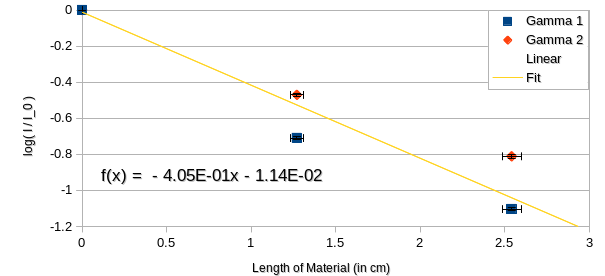
\includegraphics[width=\linewidth]{Attenuation511Al}
			\caption{The following graph shows the number of counts in their respective detector as a function of the thickness of the material in between the source and the detector. The slope tells us the attenuation coefficient of the material.}
			\label{fig:511Al}
         \end{center}
    \end{figure}  

    \begin{table}[!hbt]
      \begin{center}
        \normalsize{Attenuation Through Aluminium for 1275 keV Photon}
        \begin{tabular}{|c|c|c|c|c|}	
			\hline        	
			Detector & Thickness (cm) & Intensity & $ln(I/I_0$) & $\epsilon$ \\
            \hline
            \multirow{3}{*}{Gamma 1} & 0 & 6416 & 0 & 0.0088 \\
            \hhline{~----}
	        & 1.270 & 4424 & -0.372 & 0.014 \\
	        \hhline{~----}
            & 2.540 & 3835 & -0.515 & 0.016 \\
            \hline
            \multirow{3}{*}{Gamma 2} & 0 & 3534 & 0 & 0.011 \\
            \hhline{~----}
            & 1.270 & 2866 & -0.210 & 0.019 \\
            \hhline{~----}
            & 2.540 & 2394 & -0.389 & 0.023 \\
            \hline
       \end{tabular}
       \caption{The intensity is simply the number of incidences detected by our detector. $I_0$ is the intensity with no material in between the source and detector. $\epsilon$ is the error in log-space as defined by Eqn. (6).}
       \label{tab:aluminium1275}
      \end{center}
    \end{table}  

    \begin{figure}[!hbt]
        \begin{center}
             \normalsize{Attenuation Through Aluminium for 1275 keV Photon}
			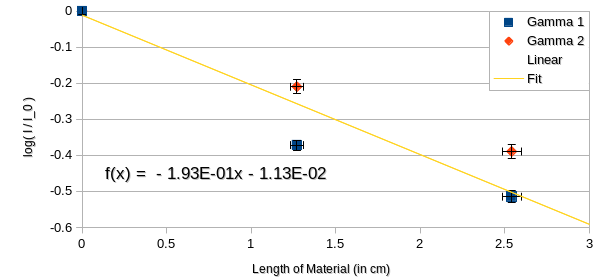
\includegraphics[width=\linewidth]{Attenuation1275Al}
			\caption{The following graph shows the number of counts in their respective detector as a function of the thickness of the material in between the source and the detector. The slope tells us the attenuation coefficient of the material.}
			\label{fig:1275Al}       
         \end{center}
    \end{figure} 

\newpage
\section{Results}

Despite it being a rough energy calibration, we expected to see a constant relationship in between samples and days. As you can see by the residuals in Figures \ref{fig:calres1} and \ref{fig:calres2}, the calibration is well outside of 5 standard deviations for numerous points. The calibration may be accurate, but it is by no means precise.
    \begin{figure}[!hbt]
        \begin{center}
			\normalsize{Gamma 1 Calibration Residuals}
			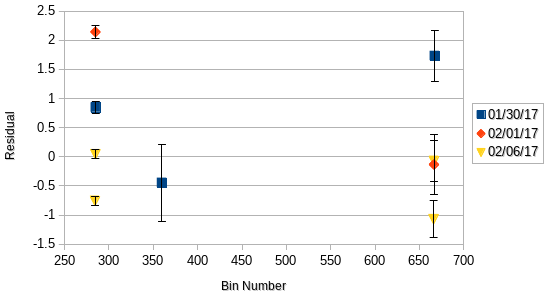
\includegraphics[width=\linewidth]{Gamma1CalResidual}
			\caption{The residuals are separated by the days they were observed. There does not appear to be a trend between the residuals on different days.}
			\label{fig:calres1}	
         \end{center}
    \end{figure}
    
    \begin{figure}[!hbt]
        \begin{center}
			\normalsize{Gamma 2 Calibration Residuals}
			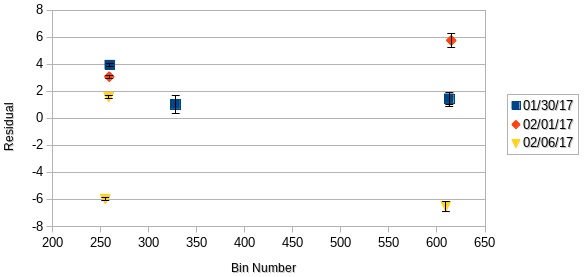
\includegraphics[width=\linewidth]{Gamma2CalResidual}
			\caption{The residuals are separated by the days they were observed. There does not appear to be a trend between the residuals on different days.}
			\label{fig:calres2}
         \end{center}
    \end{figure} 

As seen by Figure \ref{fig:511-511}, there is an obvious angular dependency for the 511 keV photons. The number of incidences around $\theta=180^\circ$ is far larger than any possible statistical fluctuation. The fluctuations in the coincidences in Figures \ref{fig:511-1275} and \ref{fig:1275-511} can be explained statistically. Therefore the 1275 keV and 511 keV photons can be considered independent of one another.

The accepted values for the attenuation coefficients for Copper are 0.7420cm$^{-1}$ for the 511 keV photons and 0.4972cm$^{-1}$ for the 1275 photons. The accepted values for Aluminium are 0.2260cm$^{-1}$ for the 511 keV photons and 0.1562cm$^{-1}$ for the 1275 keV photons\cite{nist}. Performing a least-squares linear regression on the values from Tables \ref{tab:copper511}, \ref{tab:copper1275}, \ref{tab:aluminium511}, and \ref{tab:aluminium1275}, we find the following attenuation coefficients:
\begin{eqnarray*}
\mu_{copper,511} = 0.7445\pm 0.0083cm^{-1}\\
\mu_{copper,1275} = 0.4896\pm 0.0077cm^{-1} \\
\mu_{aluminium,511} = 0.4053\pm 0.0025cm^{-1} \\
\mu_{aluminium,1275} = 0.1934\pm 0.0068cm^{-1} \\
\end{eqnarray*}
Both of the copper attenuation coefficients are in perfect agreement with the literature values. If we only consider Gamma 2 values for the aluminium fitting, we obtain the following values:
\begin{eqnarray*}
\mu_{aluminium,511} = 0.3291\pm 0.0038cm^{-1} \\
\mu_{aluminium,1275} = 0.1550\pm 0.0090cm^{-1} \\
\end{eqnarray*}

In this case, the the 1275 keV regime perfectly agrees with the literature values. The 511 keV regime is closer though still a significant number of standard errors away.
    \begin{figure}[!hbt]
        \begin{center}
			\normalsize{Attenuation Through Aluminium for 1275 keV Photon}
			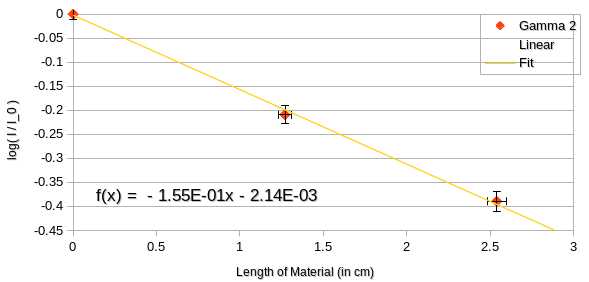
\includegraphics[width=\linewidth]{Attenuation1275Al_2}
			\caption{The following graph shows the number of counts in only the Gamma 2 detector as a function of the thickness of the material in between the source and the detector. The slope tells us the attenuation coefficient of the material. In this instance, the data is in agreement with the literature value of 0.1562cm$^{-1}$\cite{nist}.}
			\label{fig:1275al2}
         \end{center}
    \end{figure} 
\section{Conclusion}
    Using only six runs over three different days and two different radioactive materials, we were able to approximate a rough energy calibration for both of our NaI detectors. Varying the angle of the detectors we were able to clearly show an angle dependency for the 511 keV photons while the 1275 keV coincidence rates could be explained adequately by statistical fluctuations. Out attenuation coefficient for Copper in both detectors were within one standard error of the literature values. For the Aluminium sample, we were able to achieve the literature value in one detector for one of the peak despite only having six data points all of which were taken on a single day. Given the results for Copper and small sample size, we very well might have achieved more accurate results.
\section{acknowledgments}
I would like to thank my lab partners, Brandon Coleman and Taylor Grueser, who helped with the setup, data acquisition and analysis for this report.
\printbibliography

\end{document}

% This is how you include a eps figure in your document. LaTeX only accepts EPS or TIFF files.
%    \begin{figure}[!hbt]
        % Center the figure.
%        \begin{center}
        % Include the eps file, scale it such that it's width equals the column width. You can also put width=8cm for example...
%        \includegraphics[width=\columnwidth]{}
        % Create a subtitle for the figure.
%       \caption{Simulation results on the AWGN channel. Average throughput $k/n$ vs $E_s/N_0$.}
        % Define the label of the figure. It's good to use 'fig:title', so you know that the label belongs to a figure.
%        \label{fig:tf_plot}
%        \end{center}
%    \end{figure}

    % This is how you define a table: the [!hbt] means that LaTeX is forced (by the !) to place the table exactly here (by h), or if that doesnt work because of a pagebreak or so, it tries to place the table to the bottom of the page (by b) or the top (by t).
%    \begin{table}[!hbt]
        % Center the table
%        \begin{center}
        % Title of the table
%        \caption{Simulation Parameters}
%        \label{tab:simParameters}
        % Table itself: here we have two columns which are centered and have lines to the left, right and in the middle: |c|c|
%        \begin{tabular}{|c|c|}
            % To create a horizontal line, type \hline
%            \hline
            % To end a column type &
            % For a linebreak type \\
%            Information message length & $k=16000$ bit \\
%            \hline
%            Radio segment size & $b=160$ bit \\
%            \hline
%            Rate of component codes & $R_{cc}=1/3$\\
%            \hline
%            Polynomial of component encoders & $[1 , 33/37 , 25/37]_8$\\
%            \hline
%        \end{tabular}
%        \end{center}
%    \end{table}

% You can cite a book or paper by using \cite{reference}.

% You can reference tables and figure by using the \ref{label} command. Each table and figure needs to have a UNIQUE label.
%Figures and tables should be labeled and numbered, such as in Table~\ref{tab:simParameters} and Fig.~\ref{fig:tf_plot}.
